

\input{../../2021/style/preamble4tex}
% math spaces
\ifdefined\N                                                                
\renewcommand{\N}{\mathds{N}} % N, naturals
\else \newcommand{\N}{\mathds{N}} \fi 
\newcommand{\Z}{\mathds{Z}} % Z, integers
\newcommand{\Q}{\mathds{Q}} % Q, rationals
\newcommand{\R}{\mathds{R}} % R, reals
\ifdefined\C 
  \renewcommand{\C}{\mathds{C}} % C, complex
\else \newcommand{\C}{\mathds{C}} \fi
\newcommand{\continuous}{\mathcal{C}} % C, space of continuous functions
\newcommand{\M}{\mathcal{M}} % machine numbers
\newcommand{\epsm}{\epsilon_m} % maximum error

% counting / finite sets
\newcommand{\setzo}{\{0, 1\}} % set 0, 1
\newcommand{\setmp}{\{-1, +1\}} % set -1, 1
\newcommand{\unitint}{[0, 1]} % unit interval

% basic math stuff
\newcommand{\xt}{\tilde x} % x tilde
\newcommand{\argmax}{\operatorname{arg\,max}} % argmax
\newcommand{\argmin}{\operatorname{arg\,min}} % argmin
\newcommand{\argminlim}{\mathop{\mathrm{arg\,min}}\limits} % argmax with limits
\newcommand{\argmaxlim}{\mathop{\mathrm{arg\,max}}\limits} % argmin with limits  
\newcommand{\sign}{\operatorname{sign}} % sign, signum
\newcommand{\I}{\mathbb{I}} % I, indicator
\newcommand{\order}{\mathcal{O}} % O, order
\newcommand{\pd}[2]{\frac{\partial{#1}}{\partial #2}} % partial derivative
\newcommand{\floorlr}[1]{\left\lfloor #1 \right\rfloor} % floor
\newcommand{\ceillr}[1]{\left\lceil #1 \right\rceil} % ceiling

% sums and products
\newcommand{\sumin}{\sum\limits_{i=1}^n} % summation from i=1 to n
\newcommand{\sumim}{\sum\limits_{i=1}^m} % summation from i=1 to m
\newcommand{\sumjn}{\sum\limits_{j=1}^n} % summation from j=1 to p
\newcommand{\sumjp}{\sum\limits_{j=1}^p} % summation from j=1 to p
\newcommand{\sumik}{\sum\limits_{i=1}^k} % summation from i=1 to k
\newcommand{\sumkg}{\sum\limits_{k=1}^g} % summation from k=1 to g
\newcommand{\sumjg}{\sum\limits_{j=1}^g} % summation from j=1 to g
\newcommand{\meanin}{\frac{1}{n} \sum\limits_{i=1}^n} % mean from i=1 to n
\newcommand{\meanim}{\frac{1}{m} \sum\limits_{i=1}^m} % mean from i=1 to n
\newcommand{\meankg}{\frac{1}{g} \sum\limits_{k=1}^g} % mean from k=1 to g
\newcommand{\prodin}{\prod\limits_{i=1}^n} % product from i=1 to n
\newcommand{\prodkg}{\prod\limits_{k=1}^g} % product from k=1 to g
\newcommand{\prodjp}{\prod\limits_{j=1}^p} % product from j=1 to p

% linear algebra
\newcommand{\one}{\boldsymbol{1}} % 1, unitvector
\newcommand{\zero}{\mathbf{0}} % 0-vector
\newcommand{\id}{\boldsymbol{I}} % I, identity
\newcommand{\diag}{\operatorname{diag}} % diag, diagonal
\newcommand{\trace}{\operatorname{tr}} % tr, trace
\newcommand{\spn}{\operatorname{span}} % span
\newcommand{\scp}[2]{\left\langle #1, #2 \right\rangle} % <.,.>, scalarproduct
\newcommand{\mat}[1]{\begin{pmatrix} #1 \end{pmatrix}} % short pmatrix command
\newcommand{\Amat}{\mathbf{A}} % matrix A
\newcommand{\Deltab}{\mathbf{\Delta}} % error term for vectors

% basic probability + stats
\renewcommand{\P}{\mathds{P}} % P, probability
\newcommand{\E}{\mathds{E}} % E, expectation
\newcommand{\var}{\mathsf{Var}} % Var, variance
\newcommand{\cov}{\mathsf{Cov}} % Cov, covariance
\newcommand{\corr}{\mathsf{Corr}} % Corr, correlation
\newcommand{\normal}{\mathcal{N}} % N of the normal distribution
\newcommand{\iid}{\overset{i.i.d}{\sim}} % dist with i.i.d superscript
\newcommand{\distas}[1]{\overset{#1}{\sim}} % ... is distributed as ...

% machine learning
\newcommand{\Xspace}{\mathcal{X}} % X, input space
\newcommand{\Yspace}{\mathcal{Y}} % Y, output space
\newcommand{\nset}{\{1, \ldots, n\}} % set from 1 to n
\newcommand{\pset}{\{1, \ldots, p\}} % set from 1 to p
\newcommand{\gset}{\{1, \ldots, g\}} % set from 1 to g
\newcommand{\Pxy}{\mathbb{P}_{xy}} % P_xy
\newcommand{\Exy}{\mathbb{E}_{xy}} % E_xy: Expectation over random variables xy
\newcommand{\xv}{\mathbf{x}} % vector x (bold)
\newcommand{\xtil}{\tilde{\mathbf{x}}} % vector x-tilde (bold)
\newcommand{\yv}{\mathbf{y}} % vector y (bold)
\newcommand{\xy}{(\xv, y)} % observation (x, y)
\newcommand{\xvec}{\left(x_1, \ldots, x_p\right)^\top} % (x1, ..., xp) 
\newcommand{\Xmat}{\mathbf{X}} % Design matrix
\newcommand{\allDatasets}{\mathds{D}} % The set of all datasets
\newcommand{\allDatasetsn}{\mathds{D}_n}  % The set of all datasets of size n 
\newcommand{\D}{\mathcal{D}} % D, data
\newcommand{\Dn}{\D_n} % D_n, data of size n
\newcommand{\Dtrain}{\mathcal{D}_{\text{train}}} % D_train, training set
\newcommand{\Dtest}{\mathcal{D}_{\text{test}}} % D_test, test set
\newcommand{\xyi}[1][i]{\left(\xv^{(#1)}, y^{(#1)}\right)} % (x^i, y^i), i-th observation
\newcommand{\Dset}{\left( \xyi[1], \ldots, \xyi[n]\right)} % {(x1,y1)), ..., (xn,yn)}, data
\newcommand{\defAllDatasetsn}{(\Xspace \times \Yspace)^n} % Def. of the set of all datasets of size n 
\newcommand{\defAllDatasets}{\bigcup_{n \in \N}(\Xspace \times \Yspace)^n} % Def. of the set of all datasets 
\newcommand{\xdat}{\left\{ \xv^{(1)}, \ldots, \xv^{(n)}\right\}} % {x1, ..., xn}, input data
\newcommand{\ydat}{\left\{ \yv^{(1)}, \ldots, \yv^{(n)}\right\}} % {y1, ..., yn}, input data
\newcommand{\yvec}{\left(y^{(1)}, \hdots, y^{(n)}\right)^\top} % (y1, ..., yn), vector of outcomes
\renewcommand{\xi}[1][i]{\xv^{(#1)}} % x^i, i-th observed value of x
\newcommand{\yi}[1][i]{y^{(#1)}} % y^i, i-th observed value of y 
\newcommand{\xivec}{\left(x^{(i)}_1, \ldots, x^{(i)}_p\right)^\top} % (x1^i, ..., xp^i), i-th observation vector
\newcommand{\xj}{\xv_j} % x_j, j-th feature
\newcommand{\xjvec}{\left(x^{(1)}_j, \ldots, x^{(n)}_j\right)^\top} % (x^1_j, ..., x^n_j), j-th feature vector
\newcommand{\phiv}{\mathbf{\phi}} % Basis transformation function phi
\newcommand{\phixi}{\mathbf{\phi}^{(i)}} % Basis transformation of xi: phi^i := phi(xi)

%%%%%% ml - models general
\newcommand{\lamv}{\bm{\lambda}} % lambda vector, hyperconfiguration vector
\newcommand{\Lam}{\bm{\Lambda}}	 % Lambda, space of all hpos
% Inducer / Inducing algorithm
\newcommand{\preimageInducer}{\left(\defAllDatasets\right)\times\Lam} % Set of all datasets times the hyperparameter space
\newcommand{\preimageInducerShort}{\allDatasets\times\Lam} % Set of all datasets times the hyperparameter space
% Inducer / Inducing algorithm
\newcommand{\ind}{\mathcal{I}} % Inducer, inducing algorithm, learning algorithm 

% continuous prediction function f
\newcommand{\ftrue}{f_{\text{true}}}  % True underlying function (if a statistical model is assumed)
\newcommand{\ftruex}{\ftrue(\xv)} % True underlying function (if a statistical model is assumed)
\newcommand{\fx}{f(\xv)} % f(x), continuous prediction function
\newcommand{\fdomains}{f: \Xspace \rightarrow \R^g} % f with domain and co-domain
\newcommand{\Hspace}{\mathcal{H}} % hypothesis space where f is from
\newcommand{\fbayes}{f^{\ast}} % Bayes-optimal model
\newcommand{\fxbayes}{f^{\ast}(\xv)} % Bayes-optimal model
\newcommand{\fkx}[1][k]{f_{#1}(\xv)} % f_j(x), discriminant component function
\newcommand{\fh}{\hat{f}} % f hat, estimated prediction function
\newcommand{\fxh}{\fh(\xv)} % fhat(x)
\newcommand{\fxt}{f(\xv ~|~ \thetab)} % f(x | theta)
\newcommand{\fxi}{f\left(\xv^{(i)}\right)} % f(x^(i))
\newcommand{\fxih}{\hat{f}\left(\xv^{(i)}\right)} % f(x^(i))
\newcommand{\fxit}{f\left(\xv^{(i)} ~|~ \thetab\right)} % f(x^(i) | theta)
\newcommand{\fhD}{\fh_{\D}} % fhat_D, estimate of f based on D
\newcommand{\fhDtrain}{\fh_{\Dtrain}} % fhat_Dtrain, estimate of f based on D
\newcommand{\fhDnlam}{\fh_{\Dn, \lamv}} %model learned on Dn with hp lambda
\newcommand{\fhDlam}{\fh_{\D, \lamv}} %model learned on D with hp lambda
\newcommand{\fhDnlams}{\fh_{\Dn, \lamv^\ast}} %model learned on Dn with optimal hp lambda 
\newcommand{\fhDlams}{\fh_{\D, \lamv^\ast}} %model learned on D with optimal hp lambda 

% discrete prediction function h
\newcommand{\hx}{h(\xv)} % h(x), discrete prediction function
\newcommand{\hh}{\hat{h}} % h hat
\newcommand{\hxh}{\hat{h}(\xv)} % hhat(x)
\newcommand{\hxt}{h(\xv | \thetab)} % h(x | theta)
\newcommand{\hxi}{h\left(\xi\right)} % h(x^(i))
\newcommand{\hxit}{h\left(\xi ~|~ \thetab\right)} % h(x^(i) | theta)
\newcommand{\hbayes}{h^{\ast}} % Bayes-optimal classification model
\newcommand{\hxbayes}{h^{\ast}(\xv)} % Bayes-optimal classification model

% yhat
\newcommand{\yh}{\hat{y}} % yhat for prediction of target
\newcommand{\yih}{\hat{y}^{(i)}} % yhat^(i) for prediction of ith targiet
\newcommand{\resi}{\yi- \yih}

% theta
\newcommand{\thetah}{\hat{\theta}} % theta hat
\newcommand{\thetab}{\bm{\theta}} % theta vector
\newcommand{\thetabh}{\bm{\hat\theta}} % theta vector hat
\newcommand{\thetat}[1][t]{\thetab^{[#1]}} % theta^[t] in optimization
\newcommand{\thetatn}[1][t]{\thetab^{[#1 +1]}} % theta^[t+1] in optimization
\newcommand{\thetahDnlam}{\thetabh_{\Dn, \lamv}} %theta learned on Dn with hp lambda
\newcommand{\thetahDlam}{\thetabh_{\D, \lamv}} %theta learned on D with hp lambda
\newcommand{\mint}{\min_{\thetab \in \Theta}} % min problem theta
\newcommand{\argmint}{\argmin_{\thetab \in \Theta}} % argmin theta

% densities + probabilities
% pdf of x 
\newcommand{\pdf}{p} % p
\newcommand{\pdfx}{p(\xv)} % p(x)
\newcommand{\pixt}{\pi(\xv~|~ \thetab)} % pi(x|theta), pdf of x given theta
\newcommand{\pixit}[1][i]{\pi\left(\xi[#1] ~|~ \thetab\right)} % pi(x^i|theta), pdf of x given theta
\newcommand{\pixii}{\pi\left(\xi\right)} % pi(x^i), pdf of i-th x 

% pdf of (x, y)
\newcommand{\pdfxy}{p(\xv,y)} % p(x, y)
\newcommand{\pdfxyt}{p(\xv, y ~|~ \thetab)} % p(x, y | theta)
\newcommand{\pdfxyit}{p\left(\xi, \yi ~|~ \thetab\right)} % p(x^(i), y^(i) | theta)

% pdf of x given y
\newcommand{\pdfxyk}[1][k]{p(\xv | y= #1)} % p(x | y = k)
\newcommand{\lpdfxyk}[1][k]{\log p(\xv | y= #1)} % log p(x | y = k)
\newcommand{\pdfxiyk}[1][k]{p\left(\xi | y= #1 \right)} % p(x^i | y = k)

% prior probabilities
\newcommand{\pik}[1][k]{\pi_{#1}} % pi_k, prior
\newcommand{\lpik}[1][k]{\log \pi_{#1}} % log pi_k, log of the prior
\newcommand{\pit}{\pi(\thetab)} % Prior probability of parameter theta

% posterior probabilities
\newcommand{\post}{\P(y = 1 ~|~ \xv)} % P(y = 1 | x), post. prob for y=1
\newcommand{\postk}[1][k]{\P(y = #1 ~|~ \xv)} % P(y = k | y), post. prob for y=k
\newcommand{\pidomains}{\pi: \Xspace \rightarrow \unitint} % pi with domain and co-domain
\newcommand{\pibayes}{\pi^{\ast}} % Bayes-optimal classification model
\newcommand{\pixbayes}{\pi^{\ast}(\xv)} % Bayes-optimal classification model
\newcommand{\pix}{\pi(\xv)} % pi(x), P(y = 1 | x)
\newcommand{\piv}{\bm{\pi}} % pi, bold, as vector
\newcommand{\pikx}[1][k]{\pi_{#1}(\xv)} % pi_k(x), P(y = k | x)
\newcommand{\pikxt}[1][k]{\pi_{#1}(\xv ~|~ \thetab)} % pi_k(x | theta), P(y = k | x, theta)
\newcommand{\pixh}{\hat \pi(\xv)} % pi(x) hat, P(y = 1 | x) hat
\newcommand{\pikxh}[1][k]{\hat \pi_{#1}(\xv)} % pi_k(x) hat, P(y = k | x) hat
\newcommand{\pixih}{\hat \pi(\xi)} % pi(x^(i)) with hat
\newcommand{\pikxih}[1][k]{\hat \pi_{#1}(\xi)} % pi_k(x^(i)) with hat
\newcommand{\pdfygxt}{p(y ~|~\xv, \thetab)} % p(y | x, theta)
\newcommand{\pdfyigxit}{p\left(\yi ~|~\xi, \thetab\right)} % p(y^i |x^i, theta)
\newcommand{\lpdfygxt}{\log \pdfygxt } % log p(y | x, theta)
\newcommand{\lpdfyigxit}{\log \pdfyigxit} % log p(y^i |x^i, theta)

% probababilistic
\newcommand{\bayesrulek}[1][k]{\frac{\P(\xv | y= #1) \P(y= #1)}{\P(\xv)}} % Bayes rule
\newcommand{\muk}{\bm{\mu_k}} % mean vector of class-k Gaussian (discr analysis) 

% residual and margin
\newcommand{\eps}{\epsilon} % residual, stochastic
\newcommand{\epsi}{\epsilon^{(i)}} % epsilon^i, residual, stochastic
\newcommand{\epsh}{\hat{\epsilon}} % residual, estimated
\newcommand{\yf}{y \fx} % y f(x), margin
\newcommand{\yfi}{\yi \fxi} % y^i f(x^i), margin
\newcommand{\Sigmah}{\hat \Sigma} % estimated covariance matrix
\newcommand{\Sigmahj}{\hat \Sigma_j} % estimated covariance matrix for the j-th class

% ml - loss, risk, likelihood
\newcommand{\Lyf}{L\left(y, f\right)} % L(y, f), loss function
\newcommand{\Lypi}{L\left(y, \pi\right)} % L(y, pi), loss function
\newcommand{\Lxy}{L\left(y, \fx\right)} % L(y, f(x)), loss function
\newcommand{\Lxyi}{L\left(\yi, \fxi\right)} % loss of observation
\newcommand{\Lxyt}{L\left(y, \fxt\right)} % loss with f parameterized
\newcommand{\Lxyit}{L\left(\yi, \fxit\right)} % loss of observation with f parameterized
\newcommand{\Lxym}{L\left(\yi, f\left(\bm{\tilde{x}}^{(i)} ~|~ \thetab\right)\right)} % loss of observation with f parameterized
\newcommand{\Lpixy}{L\left(y, \pix\right)} % loss in classification
\newcommand{\Lpiv}{L\left(y, \piv\right)} % loss in classification
\newcommand{\Lpixyi}{L\left(\yi, \pixii\right)} % loss of observation in classification
\newcommand{\Lpixyt}{L\left(y, \pixt\right)} % loss with pi parameterized
\newcommand{\Lpixyit}{L\left(\yi, \pixit\right)} % loss of observation with pi parameterized
\newcommand{\Lhxy}{L\left(y, \hx\right)} % L(y, h(x)), loss function on discrete classes
\newcommand{\Lr}{L\left(r\right)} % L(r), loss defined on residual (reg) / margin (classif)
\newcommand{\lone}{|y - \fx|} % L1 loss
\newcommand{\ltwo}{\left(y - \fx\right)^2} % L2 loss
\newcommand{\lbernoullimp}{\ln(1 + \exp(-y \cdot \fx))} % Bernoulli loss for -1, +1 encoding
\newcommand{\lbernoullizo}{- y \cdot \fx + \log(1 + \exp(\fx))} % Bernoulli loss for 0, 1 encoding
\newcommand{\lcrossent}{- y \log \left(\pix\right) - (1 - y) \log \left(1 - \pix\right)} % cross-entropy loss
\newcommand{\lbrier}{\left(\pix - y \right)^2} % Brier score
\newcommand{\risk}{\mathcal{R}} % R, risk
\newcommand{\riskbayes}{\mathcal{R}^\ast}
\newcommand{\riskf}{\risk(f)} % R(f), risk
\newcommand{\riskdef}{\E_{y|\xv}\left(\Lxy \right)} % risk def (expected loss)
\newcommand{\riskt}{\mathcal{R}(\thetab)} % R(theta), risk
\newcommand{\riske}{\mathcal{R}_{\text{emp}}} % R_emp, empirical risk w/o factor 1 / n
\newcommand{\riskeb}{\bar{\mathcal{R}}_{\text{emp}}} % R_emp, empirical risk w/ factor 1 / n
\newcommand{\riskef}{\riske(f)} % R_emp(f)
\newcommand{\risket}{\mathcal{R}_{\text{emp}}(\thetab)} % R_emp(theta)
\newcommand{\riskr}{\mathcal{R}_{\text{reg}}} % R_reg, regularized risk
\newcommand{\riskrt}{\mathcal{R}_{\text{reg}}(\thetab)} % R_reg(theta)
\newcommand{\riskrf}{\riskr(f)} % R_reg(f)
\newcommand{\riskrth}{\hat{\mathcal{R}}_{\text{reg}}(\thetab)} % hat R_reg(theta)
\newcommand{\risketh}{\hat{\mathcal{R}}_{\text{emp}}(\thetab)} % hat R_emp(theta)
\newcommand{\LL}{\mathcal{L}} % L, likelihood
\newcommand{\LLt}{\mathcal{L}(\thetab)} % L(theta), likelihood
\newcommand{\LLtx}{\mathcal{L}(\thetab | \xv)} % L(theta|x), likelihood
\newcommand{\logl}{\ell} % l, log-likelihood
\newcommand{\loglt}{\logl(\thetab)} % l(theta), log-likelihood
\newcommand{\logltx}{\logl(\thetab | \xv)} % l(theta|x), log-likelihood
\newcommand{\errtrain}{\text{err}_{\text{train}}} % training error
\newcommand{\errtest}{\text{err}_{\text{test}}} % test error
\newcommand{\errexp}{\overline{\text{err}_{\text{test}}}} % avg training error

% lm
\newcommand{\thx}{\thetab^\top \xv} % linear model
\newcommand{\olsest}{(\Xmat^\top \Xmat)^{-1} \Xmat^\top \yv} % OLS estimator in LM 


\begin{document}

\lecturechapter{14}{Feature Selection}
\lecture{Fortgeschrittene Computerintensive Methoden}

\begin{vbframe}{Introduction}

Feature selection deals with
\begin{itemize}
\item evaluating the influence of features on the model,
\item techniques for choosing a suitable subset of features.
\end{itemize}

% First, we motivate, state different aims of variable selection and differentiate techniques.

\begin{blocki}{Goals of feature selection:}
  \item Find the set of features which achieves optimal prediction performance. This is an optimization problem.
  \item Create models more efficiently and more cost-effectively, since fewer features are used.
  Fewer features in the model $\Longrightarrow$ faster prediction, less disk space, lower costs for ascertaining features on test data.
  \item Understand models better. Specifically, models with fewer features are easier to visualize and reason about.\linebreak \textbf{Attention}: Often a trade-off between model size and prediction performance is evident!
\end{blocki}
\end{vbframe}


\begin{vbframe}{Feature selection overview}
\begin{center}
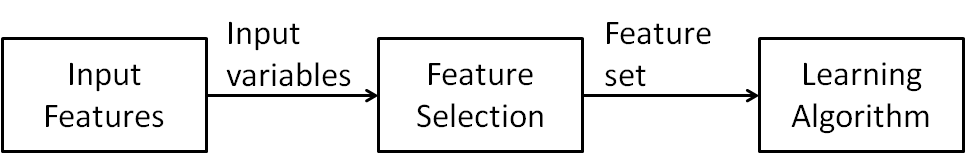
\includegraphics{figure_man/varsel_overview.png}
\end{center}

\lz

It is the task of statisticians, data analysts and machine learners to filter out the relevant information which is \textbf{useful} for prediction!
\end{vbframe}


\begin{vbframe}{Motivation Feature Selection}
\begin{itemize}
\item The information about the target class is inherent in the features.
\item Naive theoretical view:
  \begin{itemize}
  \item More features
    \begin{itemize}
    \item[$\rightarrow$] more information
    \item[$\rightarrow$] more discriminant power
    \end{itemize}
  \item Model does not care about irrelevant features anyway (e.g. by estimating their coefficients to be 0).
  \end{itemize}
\item In practice there are many reasons why this is not the case!
\item Moreover, optimizing is (usually) good, so we should optimize the input-coding.
\end{itemize}

\framebreak

\begin{itemize}
  \item In many domains we are confronted with an increasing number of features, many of which will be irrelevant or redundant, and multiple features of low quality.
  % \item This is due to the fact that there is an increasingly strong automation of measuring methods.
  % Especially the automatized collection of information by computers and the availability of information in the world wide web generates data sets with an extremely high dimensionality.
  \item In domains with many features the underlying distribution function can be very complex and hard to estimate.
  \item Irrelevant and redundant features can \enquote{confuse} learners (recall the \textbf{curse of dimensionality}).
  \item Training data are limited.
  \item Computational resources are limited.
  \item Often the usual procedures are designed for $n > p$ problems.
  \item Thus, we either need
  \begin{itemize}
    \item to adapt these procedures to high-dimensional data (e.g. by regularization),
    \item design entirely new procedures,
    \item or use the preprocessing methods addressed in this lecture.
  \end{itemize}
\end{itemize}
\end{vbframe}

\begin{vbframe}{Size of datasets}
\begin{itemize}
  \item \textbf{Classical setting}: Up to around $10^2$ features,
    feature selection might be relevant, but most of the time still manageable.
  \item \textbf{Datasets of medium to high dimensionality}:
    Around $10^2$ to $10^3$ features, basic methods still often work well.
  \item \textbf{High-dimensional data}: $10^3$ to $10^7$ features.
    Examples are e.g. micro-array / gene expression data and text categorization (bag-of-words features).

    If, in addition, observations are few, the scenario is called $p \gg n$.
\end{itemize}

\end{vbframe}

\begin{vbframe}{Feature selection vs. extraction}

\begin{columns}
%Both graphs taken out from Tim Conrad's presentation for Novisad (see cim2/external_material/tim_conrad_novisad)

\column{0.49\textwidth}
\textbf{Feature selection}

\medskip

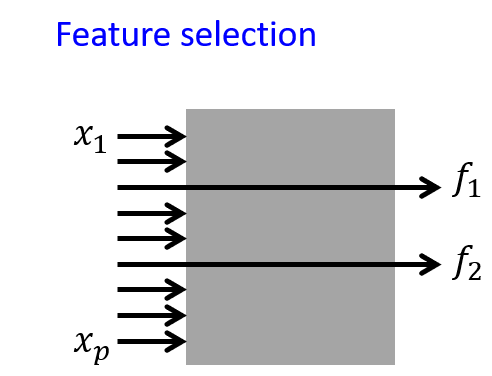
\includegraphics{figure_man/feature_selection.png}

\smallskip

\begin{itemize}
  \item Selects $\tilde{p} < p$ features.
  \item Creates a subset of the original features.
  \item Helps to understand the classification rules.
\end{itemize}

\column{0.49\textwidth}
\textbf{Feature extraction}

\medskip

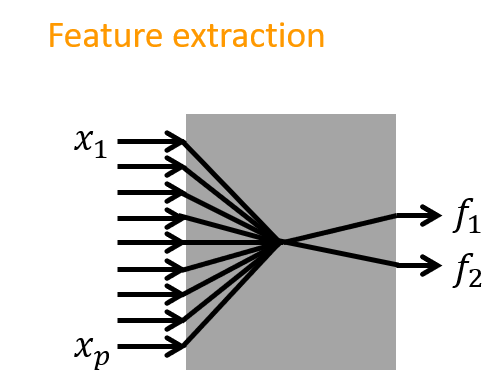
\includegraphics{figure_man/feature_extraction.png}

\smallskip

\begin{itemize}
  \item Maps inputs to $\tilde{p}$ new features.
  \item Forms linear and nonlinear combinations of the original features.
\end{itemize}

\end{columns}

% \vspace{0.3cm}
% 
% {\tiny{Source: Hsiao-Yun Huang. Regularized Double Nearest Neighbor Feature Extraction for Hyperspectral Image Classification \code{\url{https://dokumen.tips/documents/regularized-double-nearest-neighbor-feature-extraction-for-hyperspectral-image-5694e4566f1f3.html}}}\par}

\framebreak

\begin{center}
%feature_sel_vs_extr.R
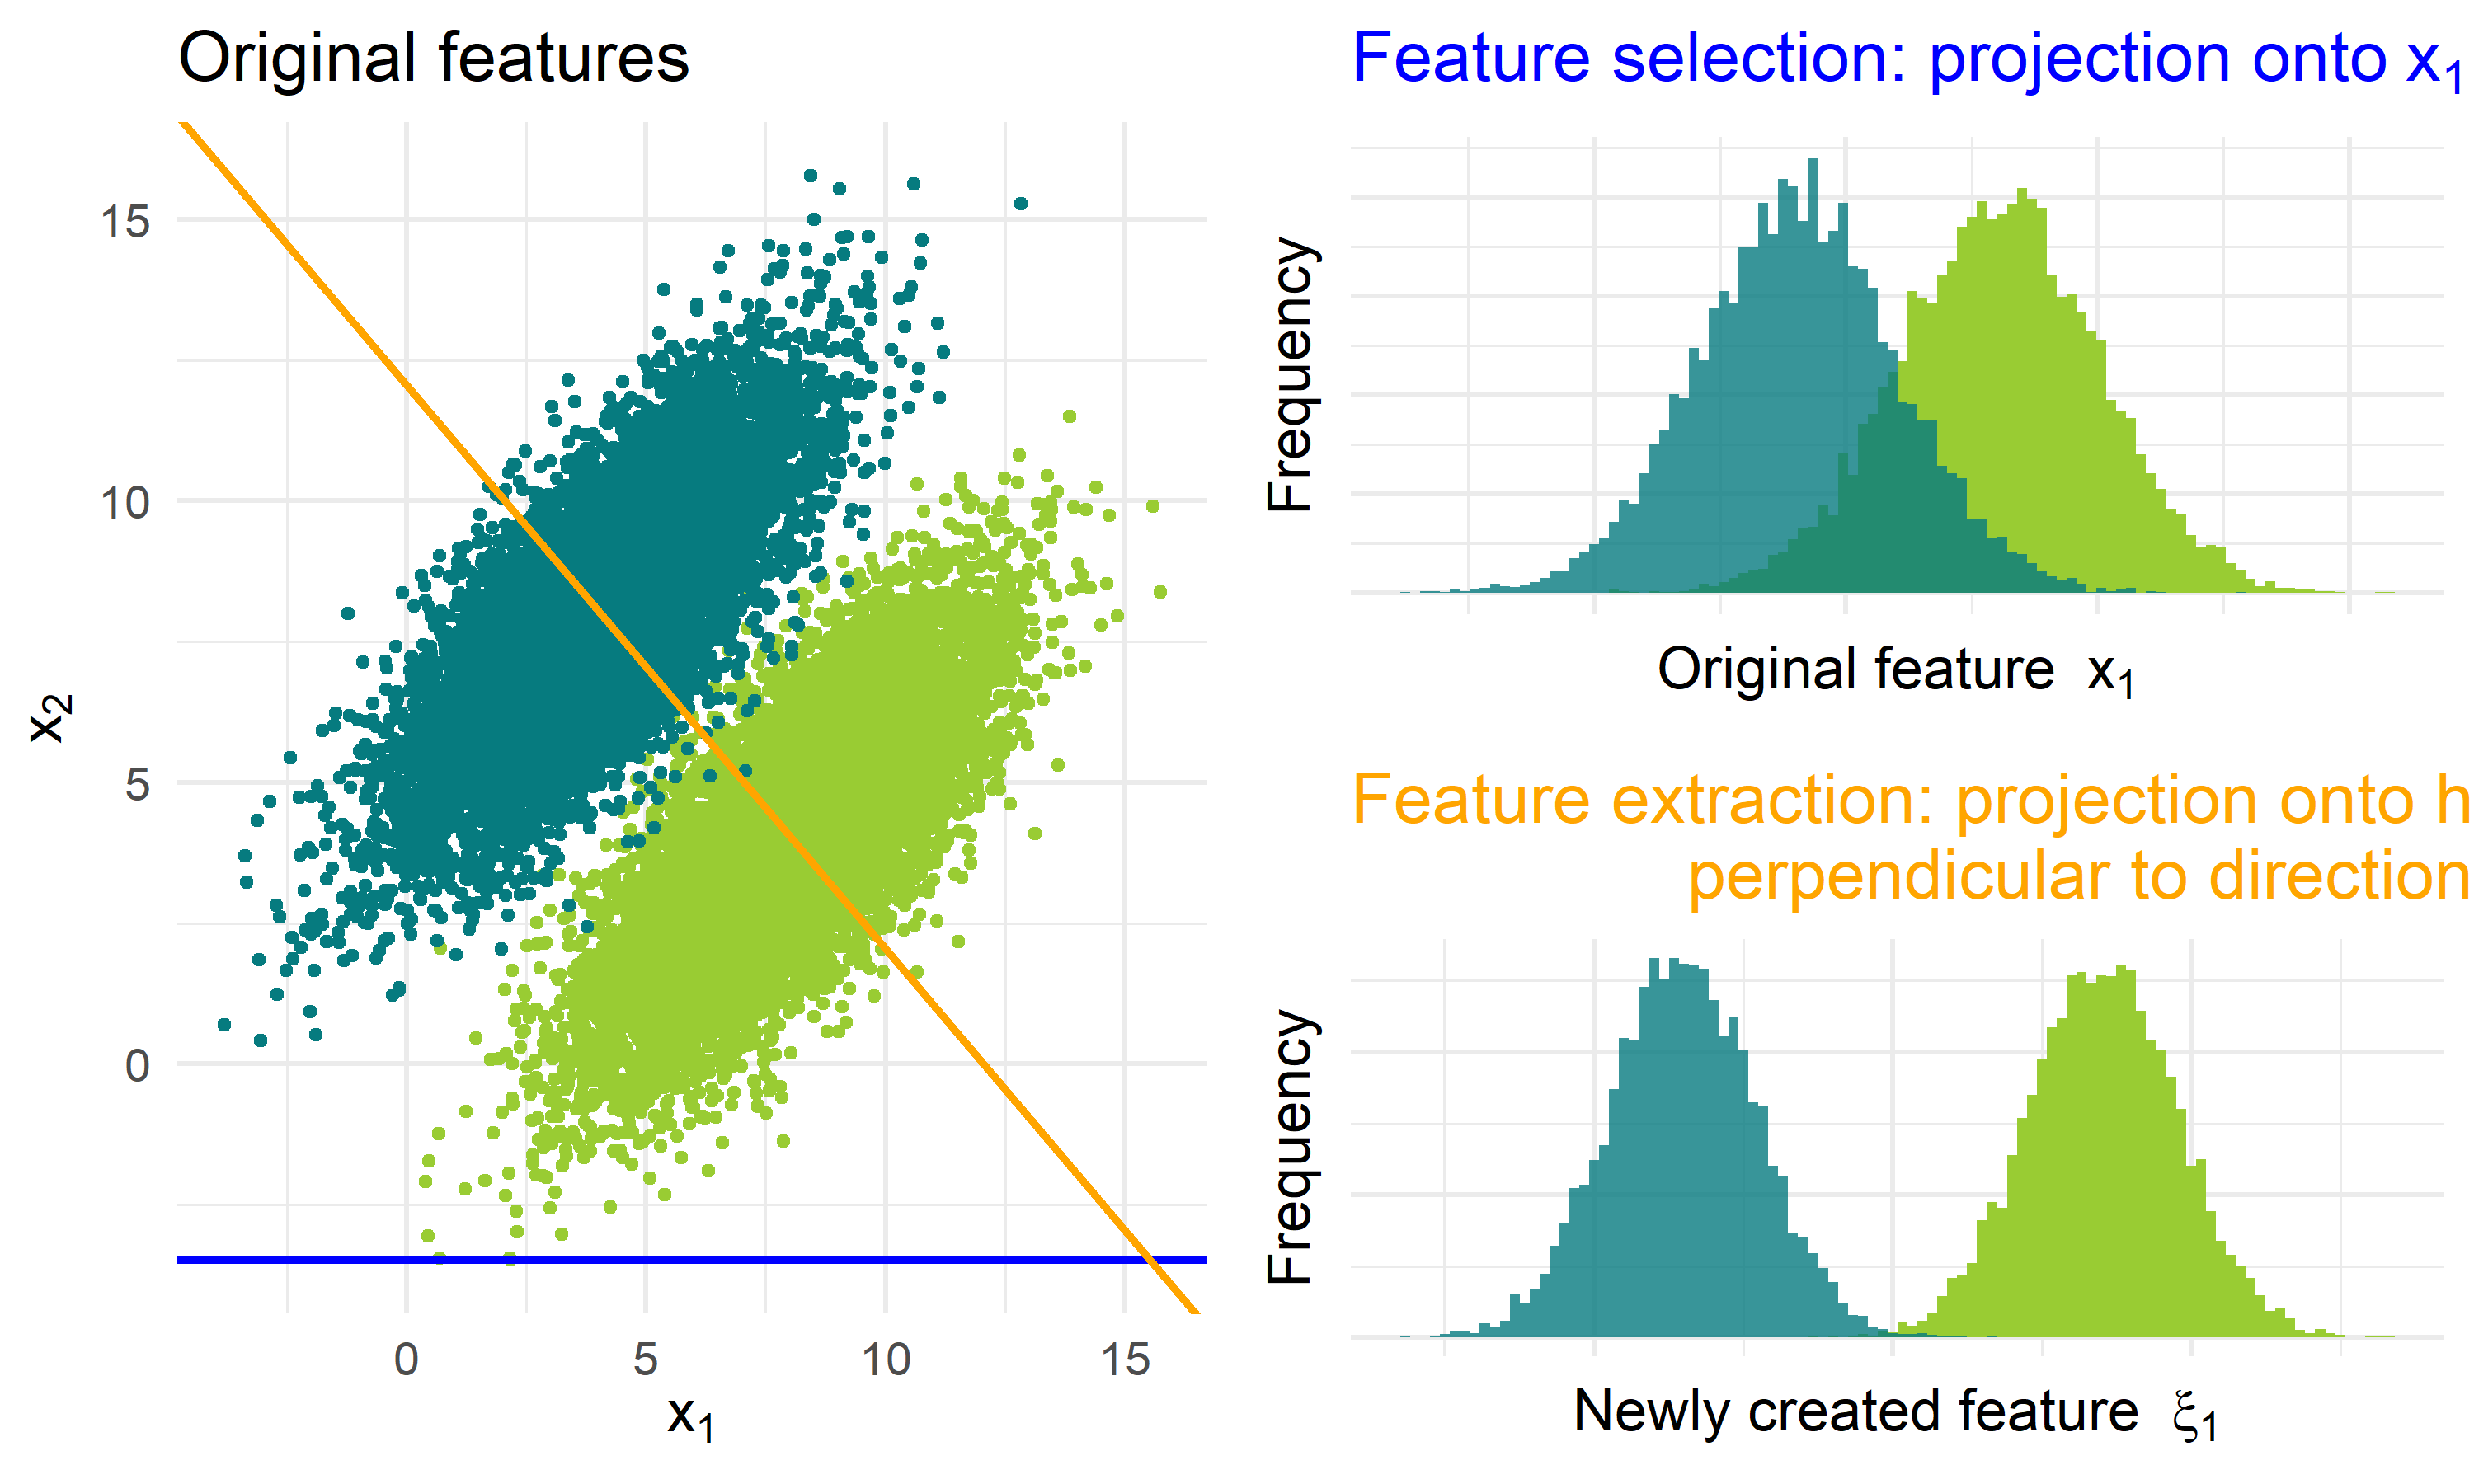
\includegraphics[width = 0.7\textwidth]{figure_man/feature_sel_vs_extr.png}
\end{center}

\footnotesize{Example for mixture of bivariate Gaussians. The projection onto the $x_1$ axis (i.e., feature selection) sees the two mixture components overlap, while projection onto the hyperplane perpendicular to the first principal component (i.e., feature extraction) separates the components.}

\normalsize

\framebreak

Both feature selection and feature extraction contribute to:

\begin{itemize}
  \item Dimensionality reduction
  \item Simplicity of classification rules
\end{itemize}

Feature extraction can be supervised (Partial Least Squares (PLS), Sufficient Dimensional Reduction (SDR)) or unsupervised (Principal Component Analysis (PCA), Multidimensional Scaling (MDS), Manifold Learning).

\end{vbframe}



\begin{vbframe}{Objective function}

\small

Given a set of features $\{1, \dots, p\}$, the feature selection problem is to find a subset $S \subset \{ 1, \dots p \}$ that
maximizes the learner's ability to classify patterns.

Formally, $\Psi^*$ should maximize some objective function
$\Psi: \Omega \rightarrow \R$:


$$\Psi^* = \argmax_{{S \in \Omega}} \{ \Psi(S) \}.$$

\begin{itemize}
\item $\Omega$ is the space of all possible feature subsets of $\{ 1, \dots, p \}$.

\item $S$ can either be a subset of features (i.e., $\Omega \subseteq \mathcal{P}(\{ 1, \dots, p \})$, $\mathcal{P}$ denoting the power set) or a bit vector (i.e., $\Omega = \{0, 1\}^p$) characterizing this subset. We will switch between those variants and the context will make clear which case we are referring to.

\item $\Psi$ can be different \enquote{things}:
  \begin{itemize}
  \small
    \item The BIC score in a linear regression model
    \item The filter score of a Minimum Redundancy Maximum Relevance (mRMR) algorithm
    \item The cross-validated test error of a learner
  
  \end{itemize}
\end{itemize}

\normalsize

\framebreak

\begin{blocki}{How difficult is it to solve the introduced optimization problem, that is, to find the optimal feature set?}
  \item The size of our search space (power set!) is $2^p$.
  \item Hence, this is a discrete optimization problem.
  \item Of course this does not mean that we have to search the entire space, since there are more efficient search strategies.
  \item Unfortunately, for the general case, it can be shown that this problem will never be perfectly and efficiently solved (NP-hard).
%  \item Formally spoken: One can show that the problem is NP-hard!
%  \item This means that the problem cannot be solved in polynomial (P) time: ${\mathcal{O}} (p^c)$, where $c \in \N$ indicates the degree o the polynom.
% \end{blocki}
% 
% \framebreak
% 
% \begin{blocki}{How difficult is it to solve the introduced optimization problem, hence, to find the optimal feature set?}
%  \item More precisely, the proof demonstrates that this problem cannot be approximated within any constant, unless P = NP.
% 
%   The latter means, that if you find an algorithm that solves a more difficult class of problems (than this optimization problem) in polynomial time, this implies that you found how to solve all easier problems (including our optimization problem) in polynomial time.
% \item \textbf{Attention}: This does not imply that it is useless trying to construct strategies which work in practice!
  \item Thus our problem now consists of moving through the search space in a smart and efficient way, thereby finding a particularly good set of features.
\end{blocki}
\end{vbframe}

% \begin{vbframe}{Motivating example: Regularization}
% \begin{itemize}
%   \item In case of $p \gg n$ \enquote{less fitting is better}.
%   \item This can be demonstrated with the following simulation study.
%   \item Investigation of three different dimensionalities of the input space: $p \in \{ 20, 100, 1000 \}$.
%   \item Data generation process for $n = 100$:
%   \begin{itemize}
%     \item $p$ random variables $X$ are sampled from a standard Gaussian distribution with pairwise correlations of 0.2.
%     \item $y$ is generated according to the linear model
%   $ y = \sum_{j=1}^p \xj \theta_j + \sigma\epsilon $, where
%     \begin{itemize}
%       \item $\epsilon$ and $\bm{\theta}$ are also sampled from standard Gaussian distributions, and
%       \item $\sigma$ is chosen such that $\var (\E[y|X]) / \sigma^2 = 2$.
%     \end{itemize}
%   \item 100 simulation runs are performed.
%   \end{itemize}
%   \item A ridge regression model with $\lambda \in \{ 0.001, 100, 1000 \}$ is fitted to the simulated data.
% \end{itemize}
% 
% \framebreak
% 
% \begin{itemize}
% \small
%   \item Boxplots show the relative test error over 100 simulations for the different values of $p$ and for the different regularization parameters $\lambda \in \{ 0.001, 100, 1000 \}$ from left to right.
%   \item Relative test error = test error / Bayes error $\sigma^2$.
%   % $\text{Relative test error} = \text{test error} / \text{Bayes error }\sigma^2$
% \normalsize
% \end{itemize}
% \begin{center}
% 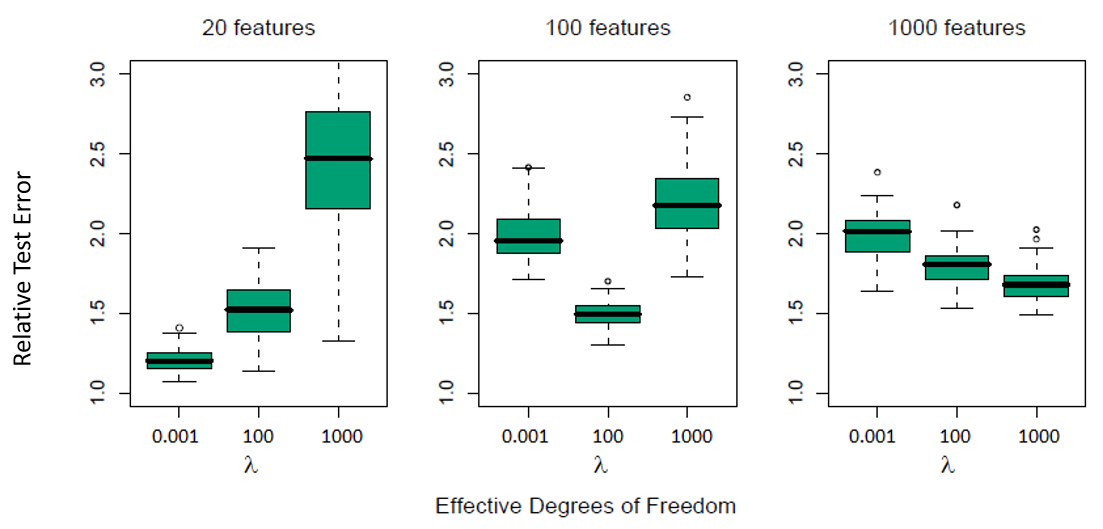
\includegraphics{figure_man/tibshirani_fig_18_1_mod.png}
% \end{center}
% 
% \tiny{Hastie (2009). The Elements of Statistical Learning. In the case of 20 features with moderate shrinkage significant coefficients are identified; with 100 features moderate shrinkage is necessary to identify some; with 1000 and therefore many nonzero coefficients, there is not much hope of finding them and we need to shrink all the way down.}
%$\rightarrow$ More regularization for high dimensional data seems reasonable.

% \begin{itemize}
% \item On the x-axis the effective degrees of freedom (averaged over the 100 simulation runs) are displayed:
% $$df(\lambda) = \sum_{j=1}^p \frac{d_j^2}{d^2_j + \lambda}$$
% where $d$ are the singular values of $x$.
% \begin{itemize}
%   \item For $\lambda = 0$ (linear regression): $df(\lambda) = p$.
%   \item For $\lambda \rightarrow \infty$: $df(\lambda) \rightarrow 0$
% \end{itemize}
% \item $\lambda = 0.001$ (20 df) has smallest relative rest error for $p = 20$.
% \item $\lambda = 100$ (35 df) has smallest relative rest error for $p = 100$.
% \item $\lambda = 1000$ (43 df) has smallest relative rest error for $p = 1000$.
% \item[$\Rightarrow$] More regularization for high dimensional data seems reasonable.
% \end{itemize}
% \end{vbframe}

\begin{vbframe}{Motivating example: Different methods}
Prediction results of eight different classification methods on micro-array data with $| \Dtrain | = 144$, $| \Dtest | = 54$, $p=16 063$ genes and a categorical target which specifies the type of cancer out of 14 different cancer types.

\begin{center}
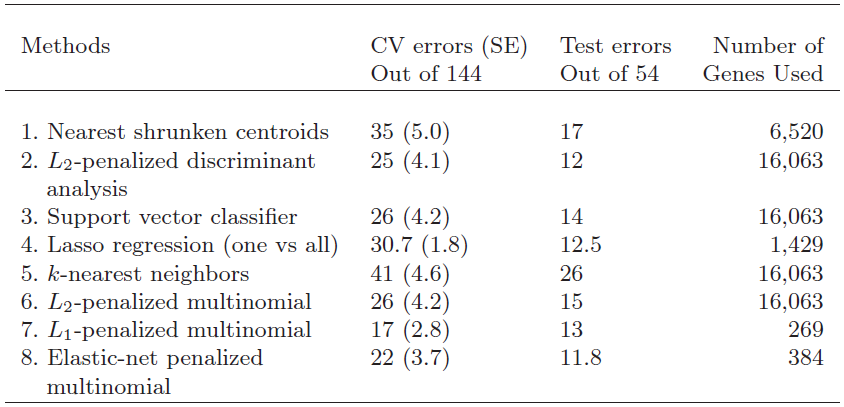
\includegraphics{figure_man/tibshirani_tab_18_1.png}

\footnotesize{Hastie (2009). The Elements of Statistical Learning}
\end{center}
\end{vbframe}

\begin{vbframe}{Motivating example: methods with integrated selection}

\begin{itemize}
\item We simulate data with function \code{sim.data} of the package \pkg{penalizedSVM}.
\item With \code{sim.data} one can simulate micro-array data.
\item Each simulated sample has \code{ng} genes.
\item \code{nsg} genes are relevant and affect the class levels.
\item The other \code{ng-nsg} have no influence.
\item The gene ratios are drawn from a multivariate normal distribution.
\end{itemize}

\framebreak

\begin{itemize}
\item Now we draw 200 observations with 50 features, 25 of which are positively and 25 are negatively correlated with the category.
\item Furthermore, we create 50 irrelevant features.
\item We compare several classification models regarding the misclassification rate.
\item Since we have relatively few data, we use repeated cross-validation with 10 folds and 10 repetitions.
\end{itemize}

\begin{table}[ht]
  \begin{center}
    \begin{tabular}{rrrrrrr}
      \hline
      & rpart & lda & logreg & nBayes & 7nn  & rForest \\
      \hline
      all feat. & 0.44 & 0.27 & 0.25 & 0.32 & 0.37 & 0.36 \\
      relevant feat. & 0.44 & 0.18 & 0.19 & 0.27 & 0.33 & 0.30 \\
      \hline
    \end{tabular}
  \end{center}
\end{table}

The models with integrated selection do not work very well here!

If we knew the relevant features, we would achieve a significant improvement.
\end{vbframe}




\begin{vbframe}{Types of feature selection methods}

In the following, we will get to know three different types of methods for feature selection:

\lz

\begin{itemize}
  \item Filters
  \item Wrappers
  \item Embedded techniques
\end{itemize}

\lz

For each technique we will look at a simple example.

\lz

It should be noted that, in practice, complicated combinations of methods can also occur.

\end{vbframe}

\endlecture
\end{document}